%%%%%%%%%%%%%%%%%%%%%%%%%%%%%%%%%%%%%%%%%%%%%%%%%%%%%%%%%
%%%%%%%%%%%%%%%%%%%%%%%%%%%%----->SECCIÓN 3<-----%%%%%%%%%%%%%%%%%%%%%%%%%
\newpage
\newpage


\chapter{Estimación del flujo de fondo de secundarios}

\noindent La colaboración LAGO estudia la influencia de la actividad solar en las variaciones del flujo de partículas secundarias, producidas durante la interacción de los rayos cósmicos con la atmósfera. Este estudio se realiza usando detectores Cherenkov de agua, o WCD. Para estudiar los datos obtenidos por estos detectores, es necesario estimar el flujo de secundarios al nivel de suelo. Dicho flujo, debe calibrarse a partir de simulaciones detalladas que tengan en cuenta todas las posibles causas de fluctuación. Para ello, se ha desarrollado una cadena de simulaciones organizadas en tres bloques principales. Como primer paso, se deben  encontrar los efectos del campo geomagnético en la propagación de partículas cargadas, que contribuyen a la radiación de fondo a nivel del suelo y que se caracterizan por la rigidez de corte en cada sitio LAGO  \citep{lagoSW}. Luego, estimar el flujo de partículas secundarias al nivel de los detectores, originado por la interacción de los primarios con la atmósfera \citep{Model}, usando el software CORSIKA  \citep{Heck1998}. Por último, obtener la respuesta del detector para los diferentes tipos de  partículas secundarias, ( \citep{andrei},  \citep{MuTe}) usando los códigos de GEANT4  \citep{GEANT4}.\\

Actualmente, para la segunda parte de la cadena de simulaciones, LAGO usa perfiles atmosféricos de la configuración ATMEXT de CORSIKA. Sin embargo, para precisar las estimaciones de flujo, se debe modelar la variabilidad de la atmósfera y establecer parámetros que permitan obtener perfiles atmosféricos precisos. Además, de ser posible hay que compararlos con los perfiles usados actualmente en cada sitio. Es por ello que el presente trabajo se concentra en la construcción y valoración de nuevos perfiles atmosféricos. A continuación, se presenta la forma como puede estimarse, el flujo de secundarios en un punto de observación determinado mediante CORSIKA, y la metodología que se usará para la obtención de estos perfiles en base al Sistema Global de Asimilación de datos GDAS.\\

%usando CORSIKA
%Por tal razón, es

\section{Flujo de fondo a nivel de Bucaramanga}

El flujo de partículas secundarias que llegan al nivel de los detectores, corresponde a la cantidad de partículas que atraviesan un área, en un nivel de observación determinado y en un intervalo de tiempo. Dicho flujo depende principalmente de dos factores: el flujo de primarios que llegan a la atmósfera, y la composición de ésta.\\

Para caracterizar el flujo de primarios se considera el flujo diferencial. Como se mencionó en el capítulo anterior, corresponde al n\'umero de astropartículas que llegan con una energía determinada $dE$ en un ángulo sólido $d\Omega$. Así, usando datos experimentales para diferentes tipos de partículas,  se puede obtener una distribución aproximada de las partículas interactuantes para un intervalo de tiempo $t$ como se muestra en la figura \ref{fig:fig8}. \\
\begin{figure}[htb!]
\centering
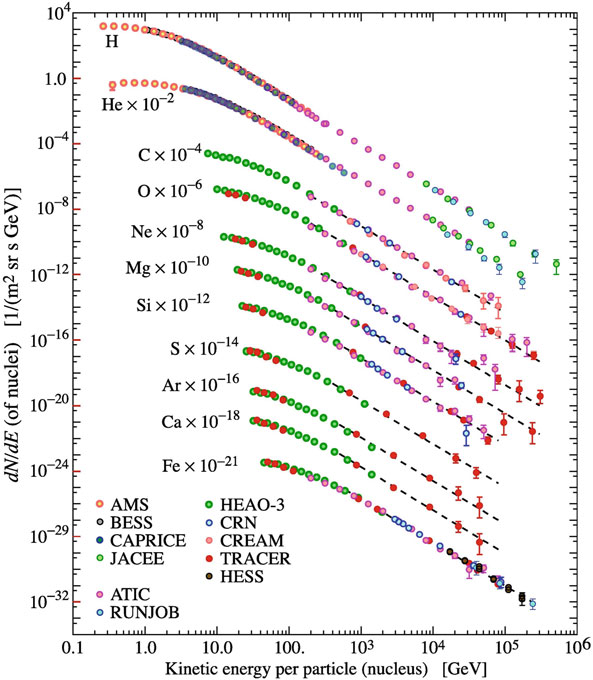
\includegraphics[width=0.5\textwidth]{Figs/differential_flux_by_nuclei.png}
\caption[Flujo de astropartículas como función de su energía.]{Flujo de núcleos de astropartículas como función de su energía  \citep{mauro:oxigen}. Los datos son tomados a partir de detecciones directas por satélites. Para mejorar la lectura de la gráfica, el flujo para cada núcleo está multiplicado por un factor de escala.}
 \label{fig:fig8}
\end{figure}

\newpage


De esta manera, se simulan individualmente cada una de los primarios. Recolectando al final, información de la totalidad de secundarios en el punto de observación. Por ejemplo, para simular un flujo en un tiempo de 120 segundos, se obtiene la siguiente distribución primarios:
\begin{table}[]
%\scriptsize
\begin{minipage}{1\textwidth}
			\caption[Distribución de primarios en un tiempo de 120 segundos.]{ \raggedright Distribución de primarios que se deben simular para estimar el flujo de secundarios en 120 s ala altura de Bucaramanga. La primera columna corresponde al código de identificación de cada núcleo en CORSIKA, la segunda el símbolo del elemento, y la tercera columna corresponde a la cantidad de núcleos que se simularán para el tiempo escogido.}
\end{minipage}
\begin{center}
\begin{tabular}{lll}
\hline
\multicolumn{1}{c}{\textbf{ID}} & \multicolumn{1}{c}{\textbf{Partícula}} & \multicolumn{1}{c}{\textbf{Cantidad}} \\ \hline
1 & H & 562322 \\ \hline
402 & He & 56595 \\ \hline
1206 & C & 1458 \\ \hline
1608 & O & 1410 \\ \hline
703 & Li & 574 \\ \hline
1105 & B & 396 \\ \hline
2412 & Mg & 335 \\ \hline
2814 & Si & 322 \\ \hline
1407 & N & 295 \\ \hline
2010 & Ne & 259 \\ \hline
5626 & Fe & 195 \\ \hline
904 & Be & 167 \\ \hline
3216 & S & 51 \\ \hline
2713 & Al & 44 \\ \hline
2311 & Na & 38 \\ \hline
4020 & Ca & 30 \\ \hline
1909 & F & 25 \\ \hline
5224 & Cr & 19 \\ \hline
4018 & Ar & 18 \\ \hline
4822 & Ti & 17 \\ \hline
5525 & Mn & 13 \\ \hline
3919 & K & 11 \\ \hline
5123 & V & 10 \\ \hline
3115 & P & 9 \\ \hline
3517 & Cl & 8 \\ \hline
4521 & Sc & 5 \\ \hline
\end{tabular}
\end{center} %\vspace{0.1em}
			\label{tab:tabla2}
\end{table}\\

\newpage

Donde la primera columna corresponde al código de identificación de cada núcleo en CORSIKA, la segunda el símbolo del elemento, y la tercera columna corresponde a la cantidad de núcleos que se simularán para el tiempo escogido. \\

Para simular el flujo de secundarios, se deben definir las condiciones iniciales. Estas deben ajustarse a las características con las que el flujo se genera de forma natural en la atmósfera. La siguiente, es la configuración con la que se realizarán las estimaciones de flujo  para este trabajo sobre la ciudad de Bucaramanga:\\


\begin{itemize}
    \item Componentes horizontal y vertical del campo magnético terrestre (en $\nu T$) correspondientes a $ 27,0263 \nu T$ y $17,176 \nu T$ respectivamente.
    \item Nivel de observación, 950 m s.n.m. para Bucaramanga.
    \item Tipo de primarios, núcleos desde el Hidrógeno hasta el Hierro.
    \item Rango de energía de los primarios: de $5GeV$ a $1\cdot 10^{6} GeV$.
    \item Ángulo cenital de incidencia de los primarios: de $0\circ$ hasta los $90\circ$.
    \item Tiempo del flujo 4 horas = $14400 s$.
    \item Tipo de detección: Volumétrica.
    \item Perfil atmosférico: Para este trabajo se usan dos tipos de perfiles atmosféricos. El perfil Subtropical dentro de las rutinas ATMEXT, que es el usado hasta ahora para las simulaciones de flujo sobre Bucaramanga, y 12 perfiles atmosféricos mensuales creados a partir de la subrutina GDASTOOL de CORSIKA cuyas características explicaremos más adelante.
\end{itemize}{}

\section{El sistema global de asimilación de datos, GDAS}

Para construir un modelo de atmósfera para CORSIKA, extraeremos datos del Sistema Global de Asimilación de Datos, GDAS \citep{GDAS_data}. Éste es un sistema de predicción numérica del clima en el que se construye un modelo que incorpora el comportamiento de la atmósfera como se encuentra en las observaciones meteorológicas. Los datos de GDAS están disponibles a través del Sistema Nacional de Archivo y Distribución de Modelos Operativos, NOAA. \\
%GDAS incluye observaciones de superficie, datos de globos aerostáticos, datos del perfil de viento, informes de aeronaves, observaciones de boya, observaciones de radar y observaciones de satélite. 

\textbf{Sistema de asimilación de datos aplicado a la atmósfera: } GDAS, realiza un ajuste de un modelo que debe describir el estado de la atmósfera para unas variables determinadas en tiempo y altura siguiendo tres pasos fundamentales:\\

1. Recolectar datos de los instrumentos que realizan observaciones meteorológicas ubicados alrededor del mundo. Estos incluyen tanto estaciones en Tierra, barcos y aviones, como radiosondas y satélites climáticos.\\

2. Utilizar el pronóstico a partir de una iteración previa del modelo, junto con la medición que describe un momento determinado. La predicción o primera estimación agrega más información al sistema, acerca del comportamiento atmosférico expresado en modelos matemáticos. \\%Los modelos usan ecuaciones diferenciales no lineales basados en termodinámica y dinámica de fluidos.\\

3. Ajustar la salida del modelo al estado atmosférico medido.\\

Un esquema que muestra esta secuencia, está representado en la figura \ref{fig:fig12}. A un tiempo dado, $ t_{0}$, las observaciones arrojan un valor de una variable de estado, y en ese mismo tiempo está disponible un pronóstico. La etapa de análisis combina observación y predicción para mejorar el modelo en $t_{0}$. Con ese ajuste, se realiza un pronóstico en un tiempo posterior $t_{1}$.

\begin{figure}[htb!]
\centering
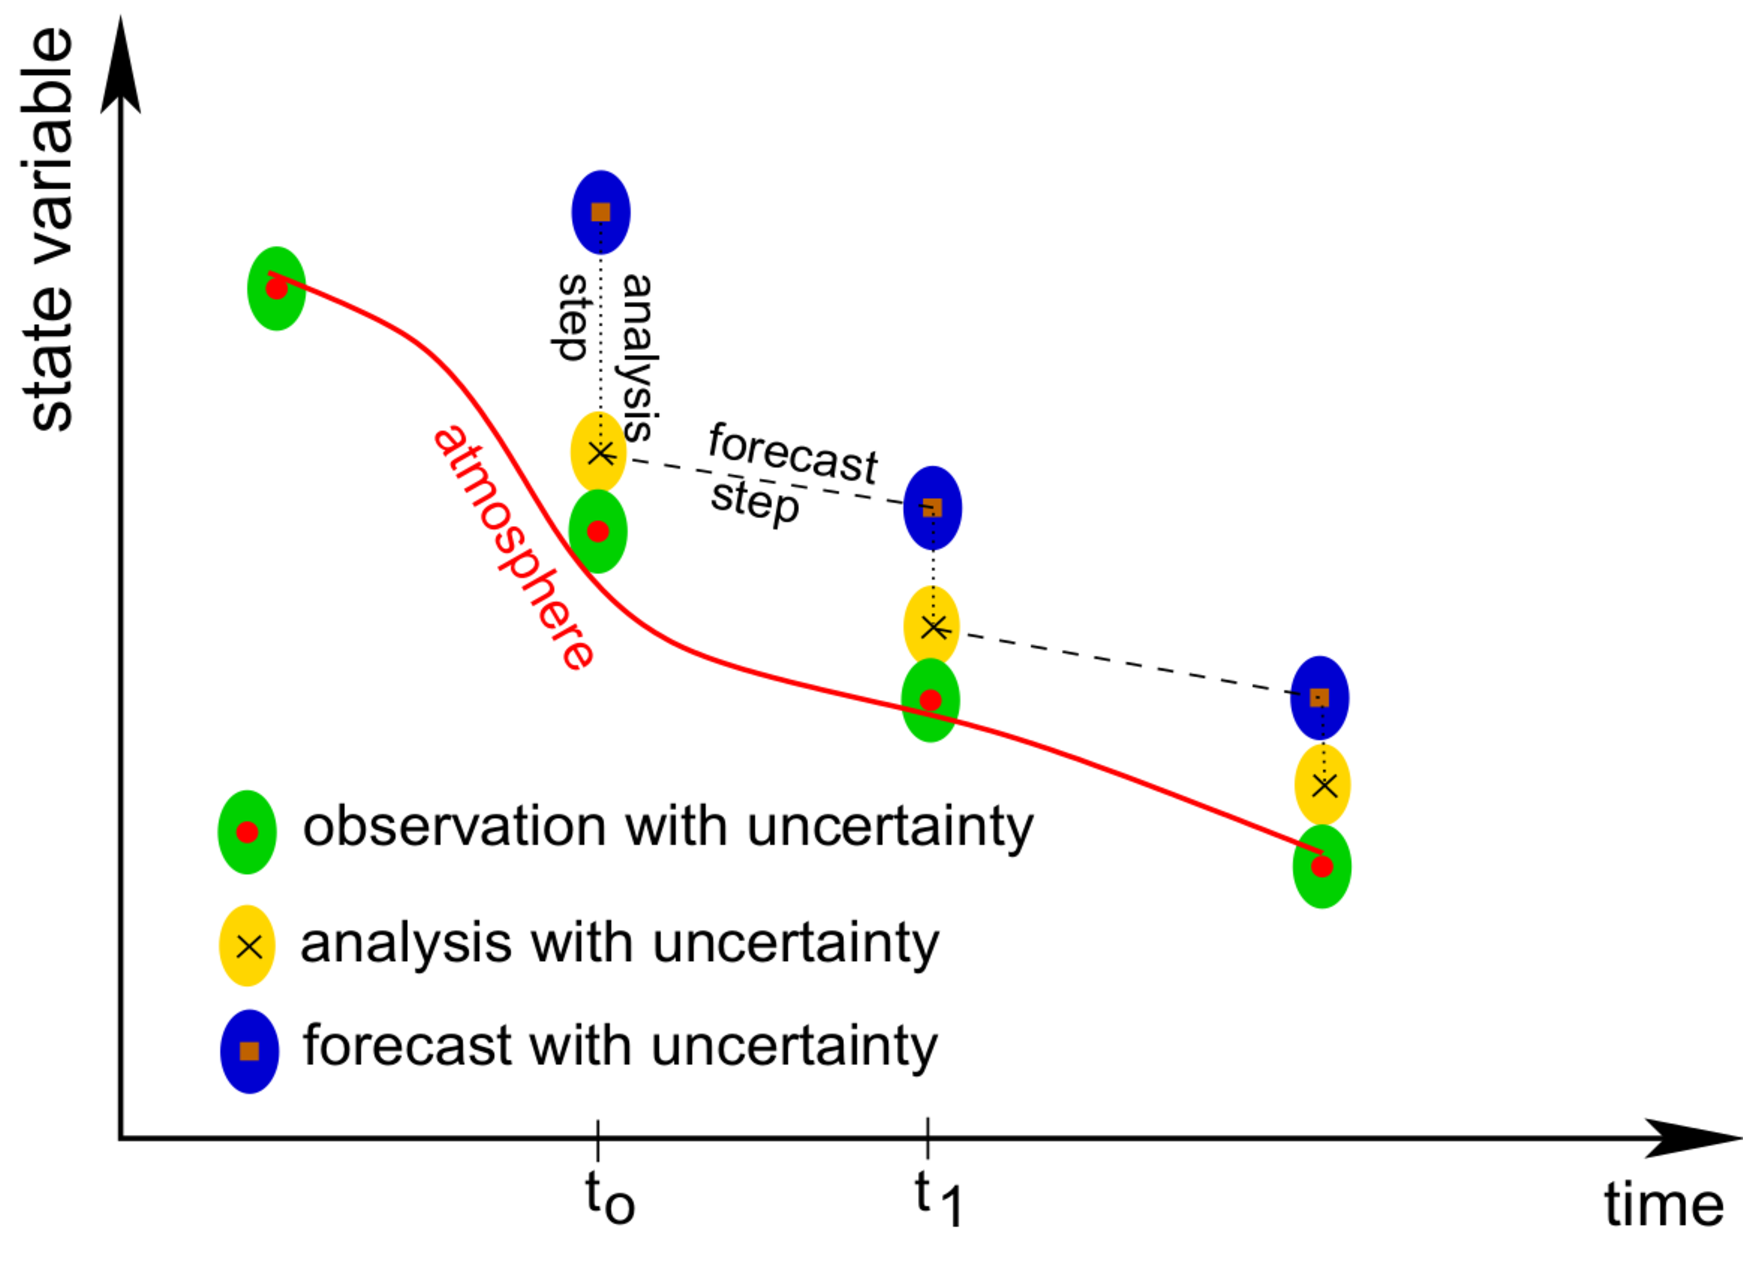
\includegraphics[width=0.55\textwidth]{Figs/gdas_data_assimilation.pdf}
\caption[Representación del método de asimilación de datos.]{Representación de la evolución y tipo de la variable de estado en el tiempo, mediante el método de asimilación de datos   \citep{GDAS_Auger}. A un tiempo dado, $ t_{0}$, las observaciones arrojan un valor de una variable de estado, y en ese mismo tiempo está disponible un pronóstico. La etapa de análisis combina observación y predicción para mejorar el modelo en $t_{0}$. Con ese ajuste, se realiza un pronóstico en un tiempo posterior $t_{1}$.}
        \label{fig:fig12}
\end{figure}
%Esta información adicional es necesaria porque las observaciones disponibles por sí solas no son suficientes.
%Un esquema que muestra el principio de la asimilación de datos está dado en la figura [3]. A un tiempo dado $t_{0}$, las observaciones proveen el valor de una variable de estado.Una predicción del modelo para esta variable desde una iteración previa existe para el mismo tiempo. El paso de análisis combina la observación con la predicción para describir el estado $t_{0}$ mejor que en la predicción anterior. Este análisis es el punto inicial para el modelo de predicción de clima para un tiempo posterior $t_{1}$.\\

%El primer paso para realizar una asimilación de datos completa es recopilar datos de instrumentos meteorológicos colocados en todo el mundo. Usando las condiciones atmosféricas en un instante determinado, un estado posterior en el tiempo se pronostica usando la predicción numérica del clima. Finalmente, la asimilación de datos se usa para ajustar la salida del modelo al estado atmosférico medido, dando como resultado una imagen tridimensional de la atmósfera. En un momento dado, el valor de una variable de estado se conoce a partir de observaciones y, para ese mismo momento, también existe un pronóstico del modelo para esta variable de una iteración anterior y así e proceso de asimilación de datos combina observación y pronóstico \citep{GDAS}.

\textbf{Contenido de los datos}: GDAS realiza un análisis cuatro veces en el día: a las 0, 6, 12 y 18 UTC, y una predicción de entre 3,6 y 9 horas. La predicción numérica del clima usada en GDAS es el Sistema de Predicción Global (GFS)  \citep{GFS}. Los datos están disponibles cada 3 horas con 23 valores de presión desde los 1000hPa gasta los los 20hPa, en una malla global de  1$^{\circ}$ en longitud y en latitud, desde enero del 2005. Estos datos son guardados en archivos semanales y están disponibles online  \citep{GDAS_data}. \\

Estudios previos, han evidenciado la confiabilidad del uso de perfiles atmosféricos construidos en base a GDAS para las estimaciones de EAS  \citep{GAP_2011}. Por esta razón, a continuación se presenta una metodología que permite la construcción y uso de perfiles atmosféricos mensuales usando esta herramienta. Esto con el fin de estudiar la sensibilidad que tiene el flujo de secundarios ante variaciones atmosféricas, para la ciudad de Bucaramanga.

\section{Creaci\'on y comparaci\'on de perfiles atmosf\'ericos mensuales}
Para construir los perfiles atmosféricos con GDAS, se ha utilizado la rutina de GDASTOOL de CORSIKA \citep{Heck1998} que extrae un perfil atmosférico para un día y hora específicas. GDASTOOL realiza la lectura de un archivo binario, del que interpreta y extrae información de la presión, altitud, temperatura y humedad, con los que realiza el cálculo de la densidad y presión atmosférica  \citep{GDAS_Auger}. Por último el código ajusta estos datos al modelo de 5 capas descrito en el capítulo anterior. Un esquema general se muestra en la figura \ref{fig:fig13}.
\begin{figure}[htb!]
\centering
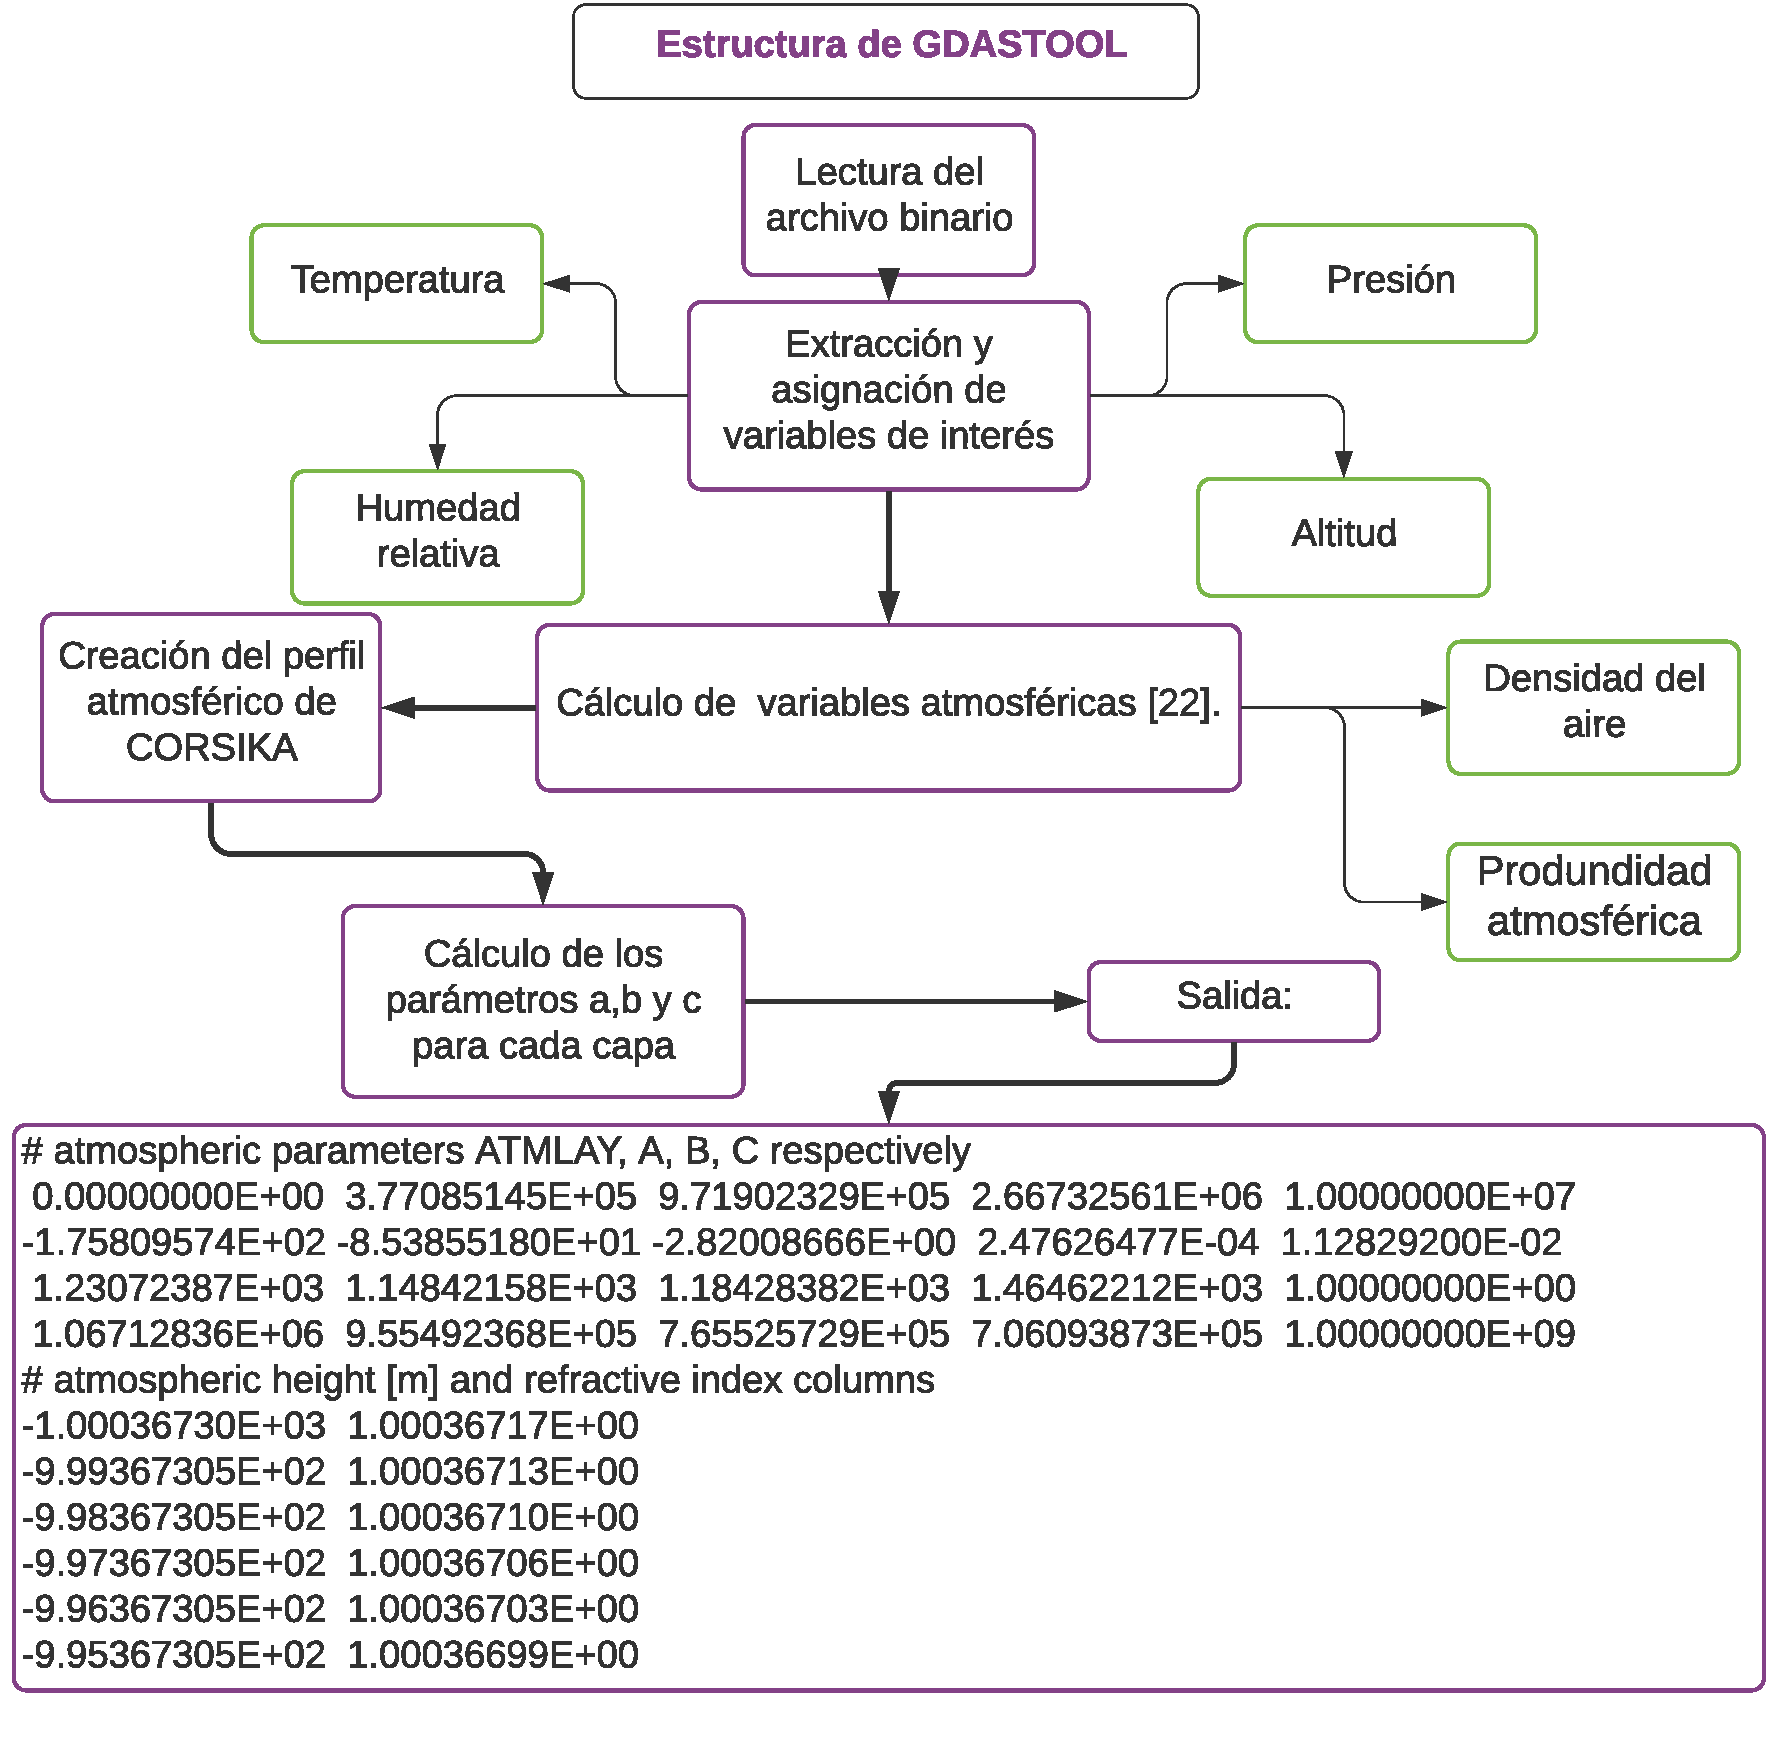
\includegraphics[width=0.85\textwidth]{Figs/GDASTOOL_code.pdf}
\caption[Esquema de GDASTOOL]{Esquema del GDASTOOL, desde la lectura del archivo binario hasta el cálculo de los parámetros $a$, $b$ y $c$ que se realiza en función de las variables atmosféricas extraídas, y las ecuaciones (\ref{eq:eq25}) y (\ref{eq:eq26}).}
 \label{fig:fig13}
 \end{figure}
%GDASTOOL ajusta estos datos a un modelo de 5 capas tal como es admitido por CORSIKA para las simulaciones, calculando los parámetros $a$, $b$ y $c$ con base en las ecuaciones (\ref{eq:eq25}) y (\ref{eq:eq26}).
\newpage
Para construir los perfiles mensuales, se ha creado un algoritmo computacional que usando el GDASTOOL, extrae datos de dos horas del día diferentes: 0:00 y las 12:00 UTC-5, para todos los días del año 2018, sobre cualquier posición geográfica, en nuestro caso, Bucaramanga (7.11 N, 73.11 E), como se observa en el esquema de la figura \ref{fig:fig14}. En total, se obtienen 730 perfiles, correspondiendo a dos perfiles por cada día del mes. En la figura \ref{fig:fig15}, se observan los primeros 62 perfiles de densidad para el mes de enero en Bucaramanga y el resultado de promediarlos para ese mes \footnote{Ver los parámetros de los 12 perfiles mensuales en el apéndice B.}.\\

\begin{figure}[htb!]
\centering
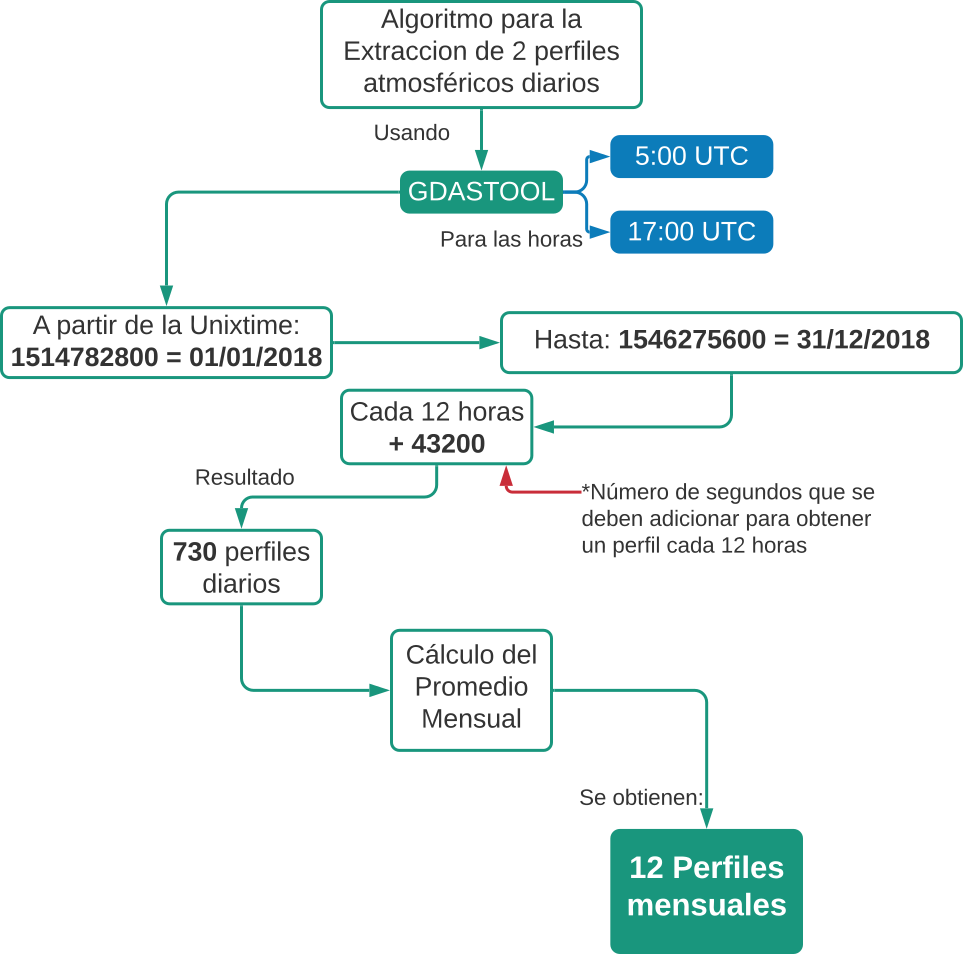
\includegraphics[width=0.9\textwidth]{Figs/Algoritmo_mensuales.pdf}
\caption[Secuencia lógica para obtener los perfiles mensuales usando GDASTOOL.]{Secuencia lógica utilizada para extraer y construir los 12 perfiles mensuales para la ciudad de Bucaramanga.}
 \label{fig:fig14}
 \end{figure}
\begin{figure}[htb!]
\centering
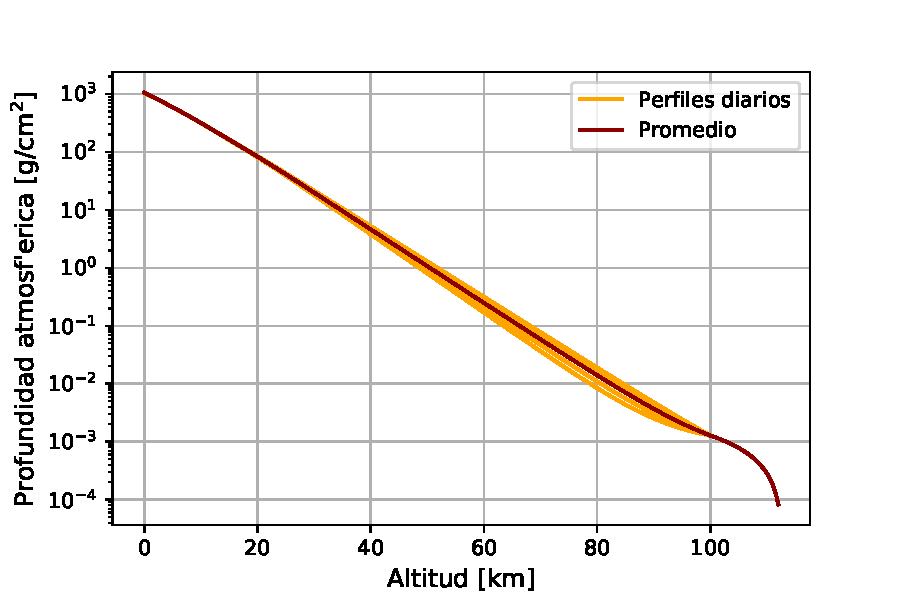
\includegraphics[width=0.8\textwidth]{Figs/promedio_enero2.pdf}
\caption[Promedio de la densidad atmosférica para la ciudad de Bucaramanga en enero.]{La figura muestra 62 perfiles de densidad para el mes de enero en Bucaramanga (líneas amarillas) y el promedio para ese mes (línea roja). Las líneas amarillas corresponden a los perfiles atmosféricos obtenidos en dos horas del día diferentes: 0:00 y las 12:00 UTC-5 durante todos los días del mes de enero, en la ciudad de Bucaramanga (7.11 N, 73.11 E). Y la línea roja corresponde al promedio de los 62 perfiles.}
\label{fig:fig15}
\end{figure}

%PÁRRAFO ADICIONAL DONDE HABLO SOBRE LA GRÁFICA DE PERFILES DIARIOS
%DIFERENCIA: 24,122503353 ABRIL Y SUBTROPICAL
De estos perfiles diarios se comienzan a observar discrepancias que se incrementan a medida que aumenta la altitud. Luego de los 100 km estas diferencias caen a cero, puesto que todos los perfiles atmosféricos tienen los mismos parámetros para esta última capa. En consecuencia, ¿Podrían observarse diferencias suficientes para justificar la creación y uso de perfiles atmosféricos mensuales, incluso en climas tropicales como el de Bucaramanga? Para dar respuesta, es necesario en primera instancia comparar los perfiles de densidad de cada uno de los meses, con los perfiles comúnmente usados para esta cuidad: el perfil Tropical y Subtropical. \\

Un contraste entre los promedios mensuales creados con GDAS, con los perfiles atmosféricos predeterminados en CORSIKA, se puede observar en la figura \ref{fig:fig16}. A la izquierda se observan todos los perfiles de densidad en los primeros 30 km. Allí, los perfiles atmosféricos subtropical y tropical se encuentran cercanos entre sí y a su vez alejados de los perfiles mensuales. Para cuantificar esta diferencia, la gráfica de la derecha muestra la diferencia entre los perfiles mensuales construidos versus el perfil subtropical. Se observa una diferencia notable que se incrementa rápidamente en los primeros 4 km hasta llegar a los 250 $g/cm^{2}$. Esto corresponde a un 58$\%$ de diferencia. Luego esta diferencia  disminuye, pero se mantiene por encima del 40$\%$.
\begin{figure}[htb!]
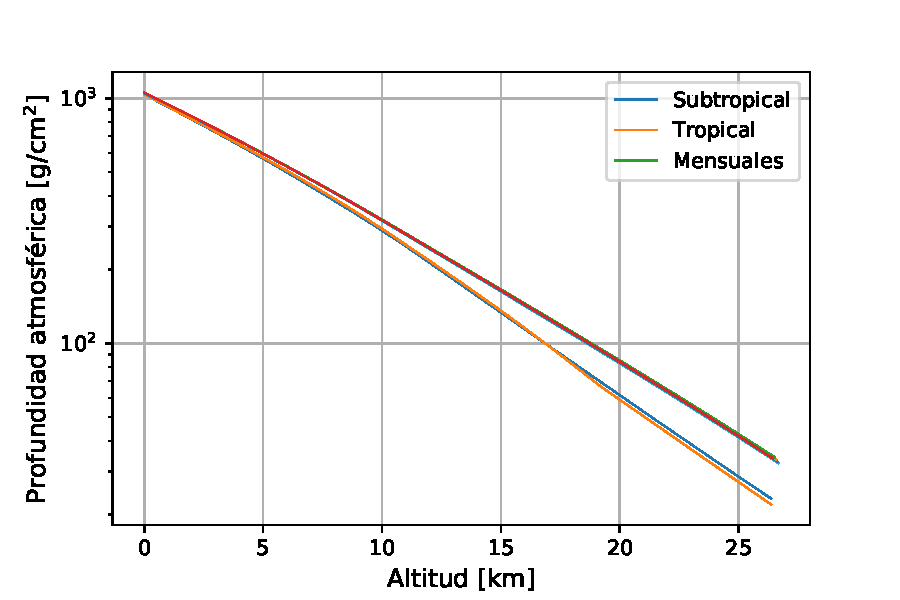
\includegraphics[width=0.4\paperwidth]{Figs/perfiles_mensuales.pdf}
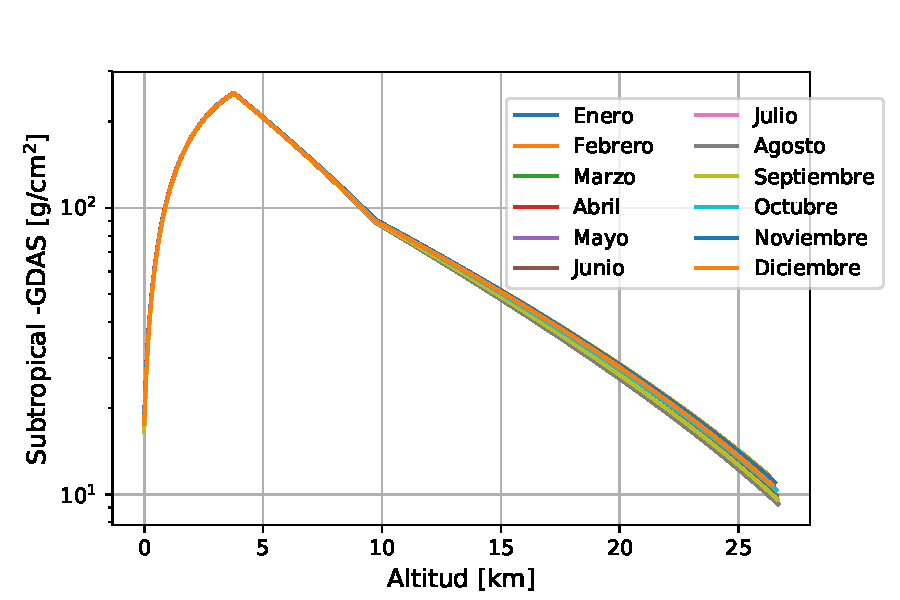
\includegraphics[width=0.4\paperwidth]{Figs/diferencias.pdf}
\caption[Promedios mensuales vs perfiles tropical y subtropical de CORSIKA.]{Contraste entre los promedios mensuales creados con GDAS, con los perfiles atmosféricos tropical y subtropical predeterminados en CORSIKA. A la izquierda se observan los perfiles de densidad para los primeros 30 km. A la derecha se observa la diferencia entre los perfiles mensuales construidos y el perfil subtropical de CORSIKA usado comúnmente para Bucaramanga. Se observa una diferencia notable que se incrementa rápidamente en los primeros 4 km hasta llegar a los 250 $g/cm^{2}$. Esto corresponde a un 58$\%$ de diferencia. Luego esta diferencia  disminuye, pero se mantiene por encima del 40$\%$.}
\label{fig:fig16}
\end{figure}

\newpage 
\section{Validaci\'on de los perfiles para la atm\'osfera de Malarg\"ue}\label{sec:ref2}

En virtud de validar la metodología implementada para la creación de perfiles atmosféricos, es necesario comprobar que los datos y aproximaciones realizadas, reproducen adecuadamente el comportamiento de la atmósfera. Esto debe realizarse para una localización previamente caracterizada, donde también se usen perfiles mensuales en base a GDAS.\\

La localización seleccionada es el Observatorio Pierre Auger, quien reemplazó los perfiles basados en mediciones con radiosondas, por perfiles atmosféricos mensuales basados en GDAS. Estos perfiles fueron construidos para la cuidad de Malarg\"ue - Argentina. Teniendo en cuenta que GDAS proporciona información diaria desde junio del 2005 hasta la fecha, este observatorio extrajo datos para dos horas del día diferentes, en todos los días disponibles, recolectando 17416 perfiles atmosféricos con los que se construyeron los promedios mensuales  \citep{GAP_2011NEW}. Las diferencias que arrojan los perfiles de GDAS con datos no superaron $1 g/cm^{2}$ como se observa en la figura \ref{fig:fig17}.\\

\begin{figure}[htb!]
\centering
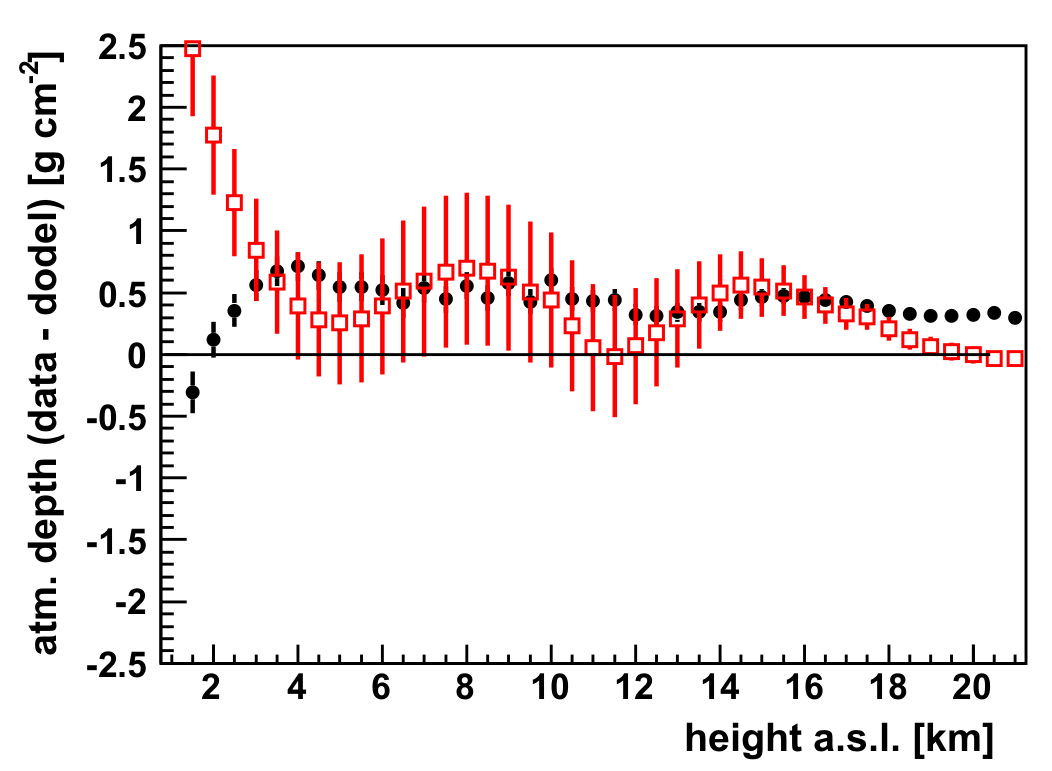
\includegraphics[width=0.7\textwidth]{Figs/nMMMvsGDAS.png}
\caption[Diferencias entre datos de radiosonda y GDAS en función de la altura.]{Diferencias entre datos de radiosonda tomados sobre Malarg\"ue  \citep{GDAS_Auger}, con los perfiles mensuales de GDAS (puntos negros) y los perfiles mensuales promedios basados en datos de radiosonda (puntos rojos) en función la altura. Para el Observatorio Pierre Auger. Las diferencias que arrojan los perfiles de GDAS con datos no superaron $1 g/cm^{2}$ como se observa en la figura \ref{fig:fig17}.}
 \label{fig:fig17}
 \end{figure}

Para realizar la validación, se construyó un perfil atmosférico para el mes de abril, entre los años 2006 y 2011, extrayendo 10 perfiles mensuales cada año en los días 6, 12, 18, 24 y 30 a las 0:00 y las 12:00 horas cada día para Malarg\"ue, usando la metodología descrita en la sección 2.3. Seguidamente, se corroboró el desarrollo de una EAS usando los dos medios de interacción, uno a la vez: la atmósfera reconstruida, y el perfil robusto de Pierre Auger. Para esto, se realizaron 100 simulaciones de un núcleo de Hierro de $1 \cdot 10^{8}$ GeV. Esta elección se hizo teniendo en cuenta que este valor de energía está en el rango de máxima eficiencia del Observatorio. \\

A partir de la figura \ref{fig:fig18} se puede observar la distribución longitudinal de partículas secundarias producto de la interacción, luego de promediar las 100 EAS bajo las mismas condiciones iniciales. Se observa que el modelo reconstruido reproduce el resultado arrojado por las atmósferas mensuales estándar de Malarg\"ue construidas con GDAS, con una diferencia porcentual por debajo del 20$\%$ después de los 400 $g/cm^{2}$. Además el comportamiento de la EAS que se obtiene con la atmósfera reconstruida muestra una diferencia de $\approx$ 2$\%$ en el valor del $X{max}$.\\

Estos resultados muestran que el método utilizado para la creación de perfiles puede reproducir las condiciones atmosféricas reales tal como lo demostró el Observatorio Pierre Auger  \citep{GDAS_Auger}. Con esto se valida la metodología implementada y los códigos utilizados,  y se procede a realizar estimaciones del flujo de secundarios con los perfiles construidos.\\

  \begin{figure}[htb!]
\centering
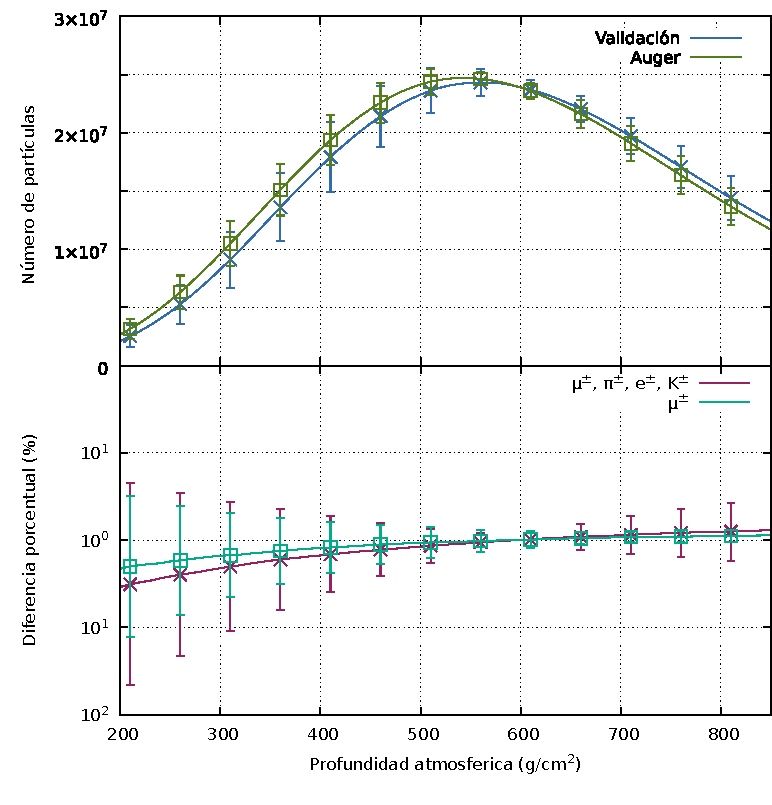
\includegraphics[width=0.8\textwidth]{Figs/longi_1E8_malargue.pdf}
\caption[Distribución longitudinal de secundarios sobre Malarg\"ue.]{Arriba, Distribución longitudinal de partículas secundarias producto de la interacción de 1 núcleo de Hierro de $1\cdot 10^{8}$ GeV sobre la atmósfera de Malargue para abril, construida por el Observatorio Pierre Auger (Verde) y la atmósfera de Malargue en abril construida mediante la metodología implementada para este trabajo (Azul). Abajo, diferencia porcentual entre las dos distribuciones longitudinales, considerando las partículas cargadas (morado) y sólo los muones (celeste). Las simulaciones consideran el mismo campo magnético y altura sobre el nivel del mar.}
 \label{fig:fig18}
 \end{figure}\\